\documentclass[
%% TIKZ_CLASSOPTION %%
tikz
]{standalone}
\usepackage{amsmath}
\usetikzlibrary{matrix}
%% EXTRA_TIKZ_PREAMBLE_CODE %%
\begin{document}
%% TIKZ_CODE %%

\usetikzlibrary{arrows,intersections}
  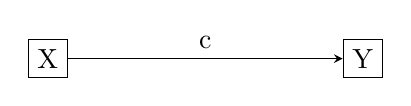
\begin{tikzpicture}
  
    \node (X) at (0,0) [draw, rectangle] {X};
    \node (Y) at (4,0) [draw, rectangle] {Y};
    
    % Arrows
    \draw[-stealth] (X) -- (Y) node[midway, above] {c};
    
  \end{tikzpicture}
\end{document}
